\documentclass[tikz]{standalone}
\usepackage{tikz}
\usetikzlibrary{decorations.pathreplacing, calc}

\begin{document}
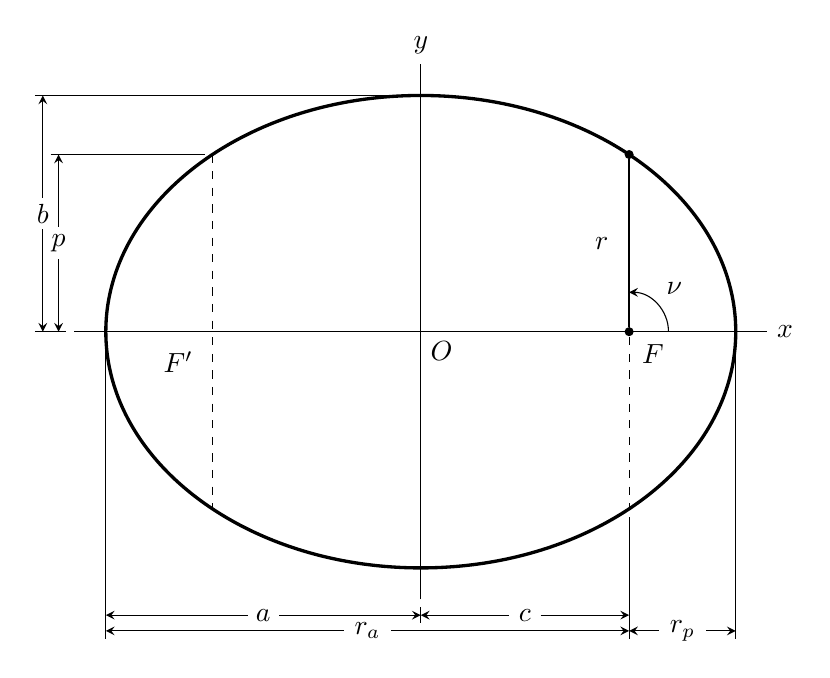
\begin{tikzpicture}[dot/.style={draw, fill, circle, inner sep=1pt}]

    % Define ellipse
    \def \a{4} % semi-major axis
    \def \b{3} % semi-minor axis
   
    
    \pgfmathsetmacro \Fx{ +sqrt(\a*\a - \b*\b) } % x-position of focal point
    \pgfmathsetmacro \e{ sqrt(1 - (\b*\b)/(\a*\a)) } % eccentricity
    \pgfmathsetmacro \p{ \a*(1 - \e*\e) }  % semi-latus rectum
    
    % Position of object in orbit
    \def \trueanomaly{90} % true anomaly in degrees
    
    \pgfmathsetmacro \r{ \p/(1 + \e*cos(\trueanomaly)) } % radius
    
    
    % Define axes
    \def \axisPadding{.4}
    \pgfmathsetmacro \xMax{ \a + \axisPadding }
    \pgfmathsetmacro \yMax{ \b + \axisPadding }
    
    % Define dimensioning
    \def \dim{.2} % dimension label margin
    
    \pgfmathsetmacro \bExtLineLeft{ -\a - .9 } % upper and lower extension line left stop
    \pgfmathsetmacro \bExtLineLwrRight{ -\a - .7 } % lower extension line right stop
    \pgfmathsetmacro \bDimX{ -\a - .8 } % bottom of lower termination arrow
    \pgfmathsetmacro \bDimLwrY{ \b/2 - \dim } % top of lower dimension line
    \pgfmathsetmacro \bDimUprY{ \b/2 + \dim } % bottom of upper dimension line
    \pgfmathsetmacro \bDimLabelY{ \b/2 } % dimension label position
    
    \pgfmathsetmacro \pExtLineLeft{ -\a - .7 } % upper and lower extension line left stop
    \pgfmathsetmacro \pExtLineUprRight{ -\Fx - .1 } % upper extension line right stop
    \pgfmathsetmacro \pExtLineLwrRight{ -\a - .5 } % lower extension line right stop
    \pgfmathsetmacro \pDimX{ -\a - .6 } % bottom of lower termination arrow
    \pgfmathsetmacro \pDimLwrY{ \p/2 - \dim } % top of lower dimension line
    \pgfmathsetmacro \pDimUprY{ \p/2 + \dim } % bottom of upper dimension line
    \pgfmathsetmacro \pDimLabelY{ \p/2 } % dimension label position
    
    \pgfmathsetmacro \aExtLineBottom{ -\b - .7 } % left and right extension line bottom stop
    \pgfmathsetmacro \aExtLineRightTop{ -\b - .5 } % right extension line top stop
    \pgfmathsetmacro \aDimY{ -\b - .6 } % leftmost of left termination arrow
    \pgfmathsetmacro \aDimLeftX{ -\a/2 - \dim } % rightmost of left dimension line
    \pgfmathsetmacro \aDimRightX{ -\a/2 + \dim } % leftmost of right dimension line
    \pgfmathsetmacro \aDimLabelX{ -\a/2 } % dimension label position
    
    \pgfmathsetmacro \cExtLineBottom{ -\b - .7 } % left and right extension line bottom stop
    \pgfmathsetmacro \cExtLineRightTop{ -\b - .5 } % right extension line top stop
    \pgfmathsetmacro \cDimY{ -\b - .6 } % leftmost of left termination arrow
    \pgfmathsetmacro \cDimLeftX{ \Fx/2 - \dim } % rightmost of left dimension line
    \pgfmathsetmacro \cDimRightX{ \Fx/2 + \dim } % leftmost of right dimension line
    \pgfmathsetmacro \cDimLabelX{ \Fx/2 } % dimension label position
    
    \pgfmathsetmacro \raExtLineBottom{ -\b - .9 } % left and right extension line bottom stop
    \pgfmathsetmacro \raExtLineRightTop{ -\p - .1 } % right extension line top stop
    \pgfmathsetmacro \raDimY{ -\b - .8 } % leftmost of left termination arrow
    \pgfmathsetmacro \raDimLeftX{ (-\a + \Fx)/2 - 1.5*\dim } % rightmost of left dimension line
    \pgfmathsetmacro \raDimRightX{ (-\a + \Fx)/2 + 1.5*\dim } % leftmost of right dimension line
    \pgfmathsetmacro \raDimLabelX{ (-\a + \Fx)/2 } % dimension label position
     
    \pgfmathsetmacro \rpExtLineBottom{ -\b - .9 } % left and right extension line bottom stop
    \pgfmathsetmacro \rpExtLineRightTop{ -.1 } % right extension line top stop
    \pgfmathsetmacro \rpDimY{ -\b - .8 } % leftmost of left termination arrow
    \pgfmathsetmacro \rpDimLeftX{ (\a + \Fx)/2 - 1.5*\dim } % rightmost of left dimension line
    \pgfmathsetmacro \rpDimRightX{ (\a + \Fx)/2 + 1.5*\dim } % leftmost of right dimension line
    \pgfmathsetmacro \rpDimLabelX{ \a + \Fx)/2 } % dimension label position 
     
    % Draw the ellipse
    \draw[very thick] (0,0) ellipse ({\a} and {\b});
    
    % Draw the x-y axes
    \draw (-\xMax, 0) coordinate[label={left:$$}] (xMin)
    -- (\xMax,0) coordinate[label={right:$x$}] (xMax);
    \draw (0, -\yMax) coordinate[label={below:$$}] (yMin)
    -- (0, \yMax) coordinate[label={above:$y$}] (yMax);
    
    % Nodes at the focal points
    \node[label={below left:$F'$}] (F2) at (-\Fx, 0) {};
    \node[dot, label={below right:$F$}] (F) at (\Fx, 0) {};
    
    % Dimensioning for b
    \draw[thin] (\bExtLineLeft, \b)  --  (0, \b); % top extension line
    
    \draw[<-, >=stealth, thin] (\bDimX, \b)  --  (\bDimX, \bDimUprY);
    \node (b) at (\bDimX, \bDimLabelY) {$ b $};
    \draw[<-, >=stealth, thin] (\bDimX, 0)  --  (\bDimX, \bDimLwrY);
    
    \draw[thin] (\bExtLineLeft, 0)  --  (\bExtLineLwrRight, 0); % bottom extension line
    
    % Dimensioning for p
    \draw[thin] (\pExtLineLeft, \p)  --  (\pExtLineUprRight, \p); % top extension line
    
    \draw[<-, >=stealth, thin] (\pDimX, \p)  --  (\pDimX, \pDimUprY);
    \node (p) at (\pDimX, \pDimLabelY) {$ p $};
    \draw[<-, >=stealth, thin] (\pDimX, 0)  --  (\pDimX, \pDimLwrY);
    
    \draw[thin] (\pExtLineLeft, 0)  --  (\pExtLineLwrRight, 0); % bottom extension line
    
    % Dimensioning for a   
    \draw[thin] (-\a, 0)  --  (-\a, \aExtLineBottom);
    
    \draw[<-, >= stealth, thin] (-\a, \aDimY)  --  (\aDimLeftX, \aDimY);
    \node (a) at (\aDimLabelX, \aDimY) {$ a $};
    \draw[->, >= stealth, thin] (\aDimRightX, \aDimY)  --  (0, \aDimY);
    
     \draw[thin] (0, \aExtLineRightTop)  --  (0, \aExtLineBottom);
     
     % Dimensioning for c   
    
    \draw[<-, >= stealth, thin] (0, \cDimY)  --  (\cDimLeftX, \cDimY);
    \node (c) at (\cDimLabelX, \cDimY) {$ c $};
    \draw[->, >= stealth, thin] (\cDimRightX, \cDimY)  --  (\Fx, \cDimY);
        
    % Dimensioning for apoapsis
    \draw[thin] (-\a, \raExtLineBottom)  --  (-\a, \aExtLineBottom);
    
    \draw[<-, >= stealth, thin] (-\a, \raDimY)  --  (\raDimLeftX, \raDimY);
    \node (ra) at (\raDimLabelX, \raDimY) {$ r_{a} $};
    \draw[->, >= stealth, thin] (\raDimRightX, \raDimY)  --  (\Fx, \raDimY);
    
     \draw[thin] (\Fx, \raExtLineBottom)  --  (\Fx, \raExtLineRightTop);
    
    % Dimensioning for periapsis 
    \draw[thin] (\a, \rpExtLineRightTop)  --  (\a, \rpExtLineBottom);
    
    \draw[<-, >= stealth, thin] (\a, \rpDimY)  --  (\rpDimRightX, \rpDimY);
    \node (rp) at (\rpDimLabelX, \rpDimY) {$ r_{p} $};
    \draw[<-, >= stealth, thin] (\Fx, \rpDimY)  --  (\rpDimLeftX, \rpDimY);
    
    % Label the origin
    \coordinate[label={below right:$O$}] (O) at (0,0);
    
    % Draw semi-latus rectum
    \draw[dashed] (\Fx, \p)  --  (\Fx, -\p);
    \draw[dashed] (-\Fx, \p)  --  (-\Fx, -\p);
    
    % Node on the ellipse, connected to foci
    \node[dot,label={\trueanomaly:$$}] (X) at ([shift=({\trueanomaly:\r})]F) {};
    
    % Draw radius to edge of ellipse
    \draw[thick] (X) -- (F) node [midway, label={\trueanomaly+90:$r$}] {};
    
    % Brace
    %\draw[decorate,decoration={brace,amplitude=5pt,mirror}] (0,\b) -- (O);
    
    % Arc for true anomaly ([shift=(starting angle:radius)]x,y center of arc coordinate) arc (starting angle:ending angle:radius)
    \draw[->,>=stealth] ([shift=(0:0.5cm)]F) arc (0:{\trueanomaly}:0.5cm) node [midway, above right] {$\nu$};

\end{tikzpicture}
\end{document}